\chapter{Implementation}
\label{chapter4}

\section{Game Implementation}
This section will outline how the game designs in section 3.2 in the design chapter were implemented and their justification. The programming language used was C++ because it is known for its wide usage in commercial games. One of the main advantages of using C++ is that is a low level language which gives more performance and performance is an important factor in games. 
\newline
\par
Another reason that C++ is used is that it supports many libraries and one of the libraries that is supported is OpenGL. OpenGL stands for Open Graphics Library and is used to render 3D graphics and supports multiple platfroms (Windows, Linux, OSX) \cite{opengl}. Since OpenGL only deals with 3D rendering, Qt is used as a framework to help build the game. Qt is a framework that is used to develop applications which also supports multiple platforms like OpenGL \cite{qt}. Qt has an OpenGL module to make developing in OpenGL easier and can takes advantage of the whole Qt API for non-OpenGL specifc functionality such as networking which will be explained in section 4.2.
\newline
\par
As shown in Figure \ref{fig:game}, a procedurally generated tree is being modelled along with lighting and shadows. The interface controls on the side are used for testing such as moving the tree to test the shadow and increasing the complexity of the tree. Frames per second counter is implemented and is outputted in the terminal as shown in \ref{fig:gamefps}. The flight simulator can be controlled using the following keyboard commands:
\begin{itemize}
 \item W / S		-	Accelerate / Decelerate
 \item Q / E 		-	Roll Left / Roll Right
 \item Up / Down 	-	Pitch Down / Pitch Up
 \item Left / Right	-	Yaw Left / Yaw Right
 \item Space		-	Stop Movement
 \item F 			-	Toggle FPS counter
\end{itemize}

\begin{figure}[h!]
 \centering
 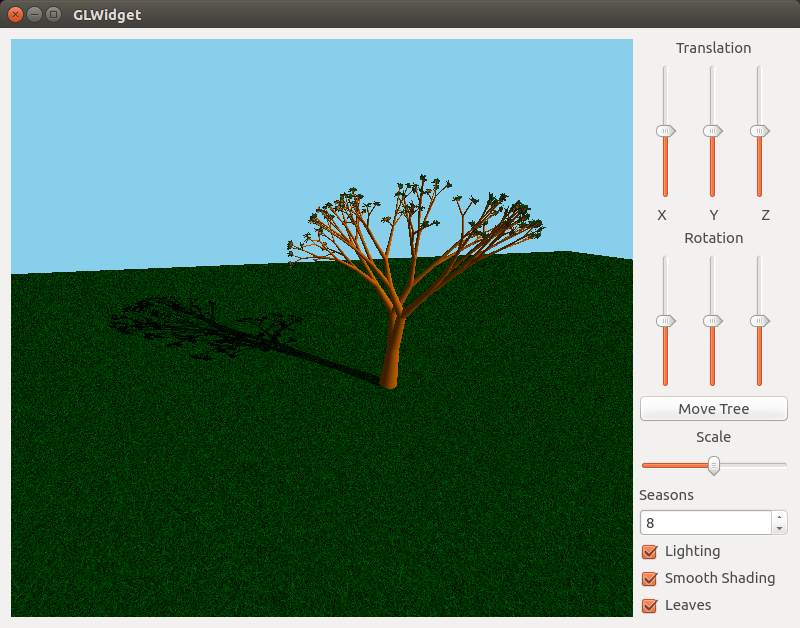
\includegraphics[width=\linewidth]{images/game.png}
 \caption{Screenshot of game with a procedurally generated tree}
 \label{fig:game}
\end{figure}

\begin{figure}[h!]
 \centering
 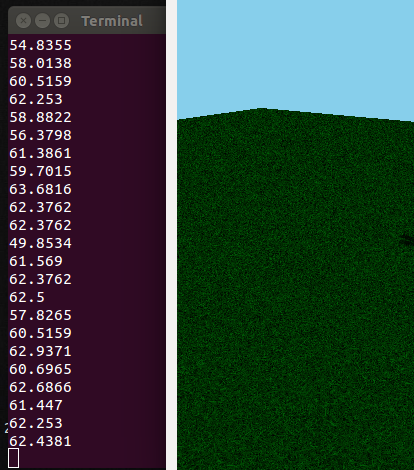
\includegraphics[width=0.5\linewidth]{images/gamefps.png}
 \caption{Screenshot of frames per second beind display in the terminal}
 \label{fig:gamefps}
\end{figure}

\section{Cloud Gaming}
The basic cloud gaming system implementation uses Qt's framework for the networking in terms of client and server connection. Since Qt was already used for OpenGL, using Qt for networking will make communication easier. The client program is simply a Qt program that connects to the server program through IP address and port number using Qt's networking module. Once a connection is made, a Qt window appears that will listen to keyboard commands from the user. Only commands that is mapped for the flight simulator controls is accepted as well as held keys being taken in to account then these commands are sent to the server. The server accepts these inputs and simulates the game commands so the game engine can process them to produce the next frames as shown in Figure \ref{fig:gamecommands}.

\begin{figure}[h!]
 \centering
 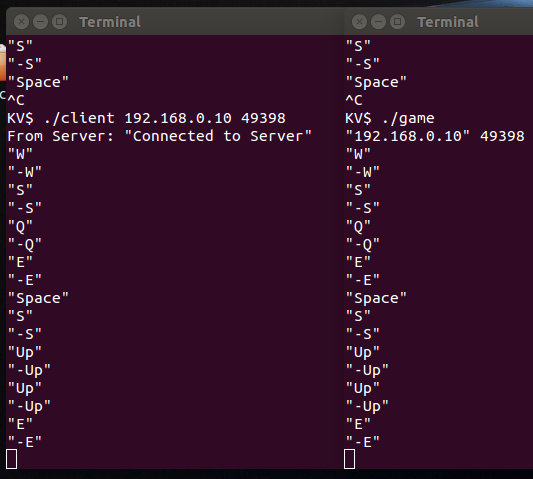
\includegraphics[width=0.7\linewidth]{images/gamecommands.png}
 \caption{Screenshot of client connection to server and sent commands}
 \label{fig:gamecommands}
\end{figure}

Due to time constraints and setbacks, the video streaming portion of the cloud gaming system was not completed and I will outline the initial implementation plans. The rendered frames on the server side needed to be rendered off screen so it will not display on the server machine. This is done by using Qt's QOffscreenSurface class that allows rendering with OpenGL on an arbitrary thread without the need to create a QWindow then these offscreen rendered frames are then captured in to QImage format \cite{qoffscreen}. Capturing frames to QImage format was actually already implemented but further work on it was not carried out.
\newline
\par
The captured QImage frames are then to be encoded in to streamable H.264 MP4 video format since it is compressed so video traffic data size is smaller. This was supposed to be done using a Qt wrapper called QtFFmpegWrapper\cite{qtffmpeg} for FFmpeg which helps encode and decode video. It uses Qt QImage to exchange video frames with the encoder/decoder. Unfortunately, this code has not been updated for three years so some functions have been deprecated with recent Qt and FFmpeg versions leading to it not being able to be compiled. With the time constraints, learning the ffmpeg library to manually encode QImage data would have been too time consuming with the networking implementations and report deliverables still to be completed.
\newline
\par
The next step would have been to stream the video frames to the client using live555 library. The live555 media server is a complete RTSP (Real Time Streaming Protocol) server application \cite{live555}. The thin client program can then receive and play these video frames back to the window using Qt's media player RTSP compliant capabilities so the user can see the response of their keyboard commands.
 
\section{Networking Implementation}
The original networking implementation idea was to use the University of Leeds' School of Computing cloud testbed for testing software-defined networking in a real data centre network. Open vSwitch is an example of a virtual switch which is a software program that enables communications between virtual machines \cite{openvswitch} which makes it essential to SDN deployments in data centres. Even though the cloud testbed is capable of using Open vSwitch, it was not enabled when it was first set up which is the only time it can be enabled. The other option is to use a virtual network to simulate a network and its latencies as well as the video traffic.

\subsection{Mininet Virtual Network}
Mininet is a tool that can be used to create a virtual network on a single machine with the ability to use virtual switches such as Open vSwitch. Latencies and bandwidth limits can be set on the links between the switches to simulate real world link delays and limitations. The bandwidth limitations that is set on the links between the player hosts and the core switch of the data centre is based on the UK's average network bandwidth in different areas \cite{avgbandwidth} as shown in Table \ref{table:links}. The link delay from the players to the core switch is set to 15ms for all players since 30ms is an average ping time to a typical data centre location. The link delays in the data centre are all set to 1ms since there should be little to no latency where server machines are close to each other. Figure \ref{fig:mnnetwork} shows a diagram of the mininet virtual network along with the IP address of the hosts and port numbers of switch links as well as host and switch names for easier referencing.

\begin{table}[h!]
\centering
\begin{tabular}{|l|l|l|}
\hline
\multicolumn{1}{|c|}{\textbf{Connection}} & \multicolumn{1}{c|}{\textbf{Bandwidth}} & \multicolumn{1}{c|}{\textbf{Link Delay}} \\ \hline
\textbf{h1 -\textgreater s1}             & 70 Mbps                                 & 15 ms                                    \\ \hline
\textbf{h2 -\textgreater s1}              & 50 Mbps                                 & 15 ms                                    \\ \hline
\textbf{h3 -\textgreater s1}              & 30 Mbps                                 & 15 ms                                    \\ \hline
\end{tabular}
\caption{Table showing player host link parameters}
\label{table:links}
\end{table}

\begin{figure}[h!]
 \centering
 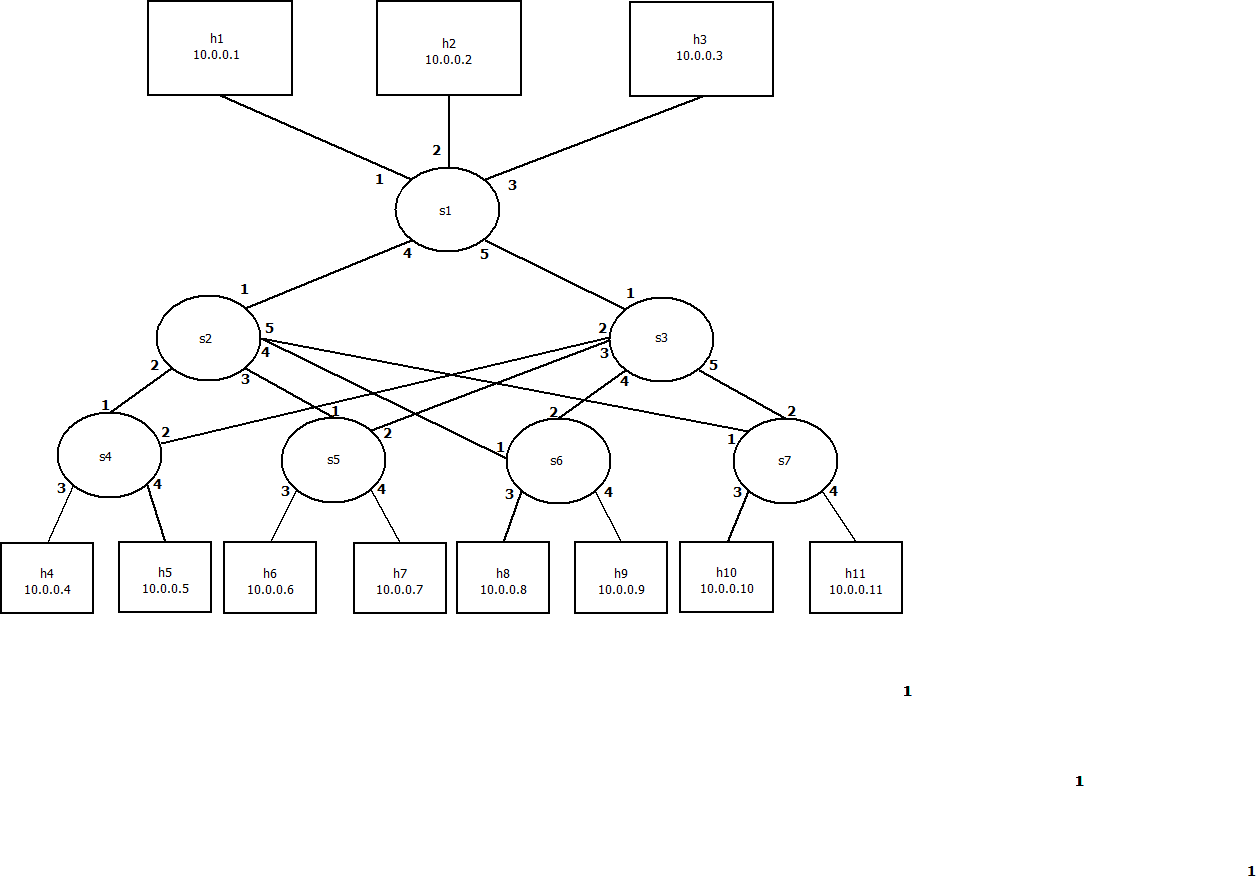
\includegraphics[width=\linewidth]{images/mnnetwork.png}
 \caption{Mininet network topology with port numbers and host names and IP address}
 \label{fig:mnnetwork}
\end{figure}



\subsection{OpenDaylight}

\subsection{Load Balancer}

\begin{figure}[h!]
 \centering
 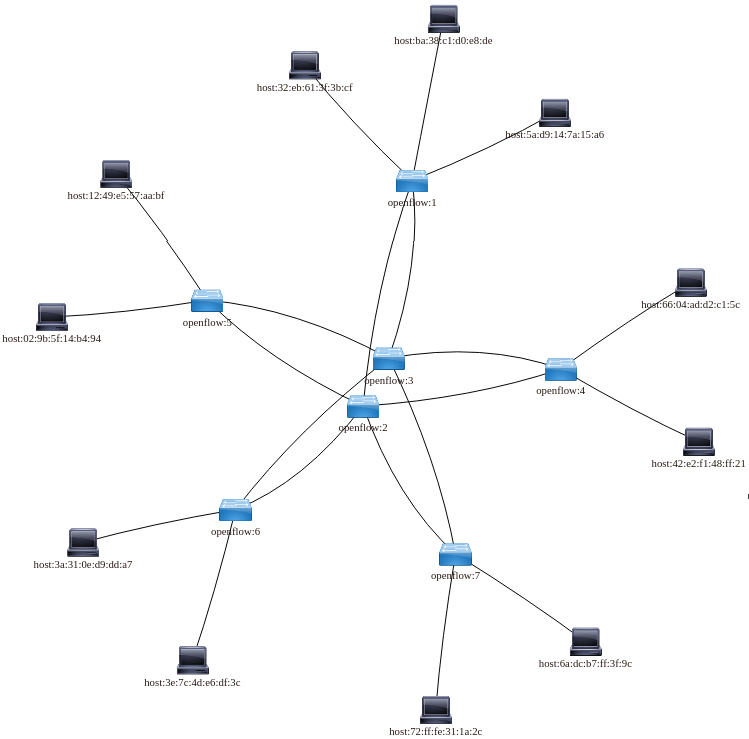
\includegraphics[width=\linewidth]{images/odltopo.png}
 \caption{OpenDaylight network topology}
 \label{fig:odltopo}
\end{figure}